\documentclass[a4paper]{article} 
\addtolength{\hoffset}{-2.25cm}
\addtolength{\textwidth}{4.5cm}
\addtolength{\voffset}{-3.25cm}
\addtolength{\textheight}{5cm}
\setlength{\parskip}{0pt}
\setlength{\parindent}{0in}

\usepackage{natbib}
\usepackage{blindtext} % Package to generate dummy text
\usepackage{charter} % Use the Charter font
\usepackage[utf8]{inputenc} % Use UTF-8 encoding
\usepackage{microtype} % Slightly tweak font spacing for aesthetics
\usepackage{amsthm, amsmath, amssymb} % Mathematical typesetting
\usepackage{float} % Improved interface for floating objects
\usepackage{hyperref} % For hyperlinks in the PDF
\usepackage{graphicx, multicol} % Enhanced support for graphics
\usepackage{xcolor} % Driver-independent color extensions
\usepackage{pseudocode} % Environment for specifying algorithms in a natural way
\usepackage[ddmmyyyy]{datetime} % Uses YEAR-MONTH-DAY format for dates
%\usepackage{gensymb}
\usepackage{bibentry}

\usepackage{fancyhdr} % Headers and footers
\pagestyle{fancy} % All pages have headers and footers
\fancyhead{}\renewcommand{\headrulewidth}{0pt} % Blank out the default header
\fancyfoot[L]{} % Custom footer text
\fancyfoot[C]{} % Custom footer text
\fancyfoot[R]{\thepage} % Custom footer text
\newcommand{\note}[1]{\marginpar{\scriptsize \textcolor{red}{#1}}} % Enables comments in red on margin

%----------------------------------------------------------------------------------------

\usepackage{adjustbox}
\usepackage{float}
\usepackage{multicol}
%-------------------------------
%	TITLE VARIABLES (identify your work!)
%-------------------------------

\newcommand{\yourname}{Jakob Kralj 4.A} % replace YOURNAME with your name
\newcommand{\papertitle}{Merjenje specifične toplote snovi} % replace X with paper title

\begin{document}

%-------------------------------
%	TITLE SECTION (do not modify unless you really need to)
%-------------------------------
\fancyhead[C]{}
\hrule \medskip
\begin{minipage}{0.295\textwidth} 
\raggedright
\footnotesize
\yourname \hfill\\ 
\end{minipage}
\begin{minipage}{0.69\textwidth} 
\centering 
\Large
\text{\papertitle}\\ 
\normalsize 
\end{minipage}
\medskip\hrule 
\bigskip


%-------------------------------
%	ASSIGNMENT CONTENT (add your responses)
%-------------------------------

\section*{Naloga:} % this is an example

Izmeri specifično toploto štirih različnih kovin in izmerjeno vrednost primerjaj z vrednostmi specifičnih toplot teh kovin, ki jih najdeš v tabelah. 

\section*{Potrebščine:}

Kalorimeter, termometer, 150 ml vode, telesa iz štirih različnih kovin, vsako ima maso 200 g.

\section*{Skica:}

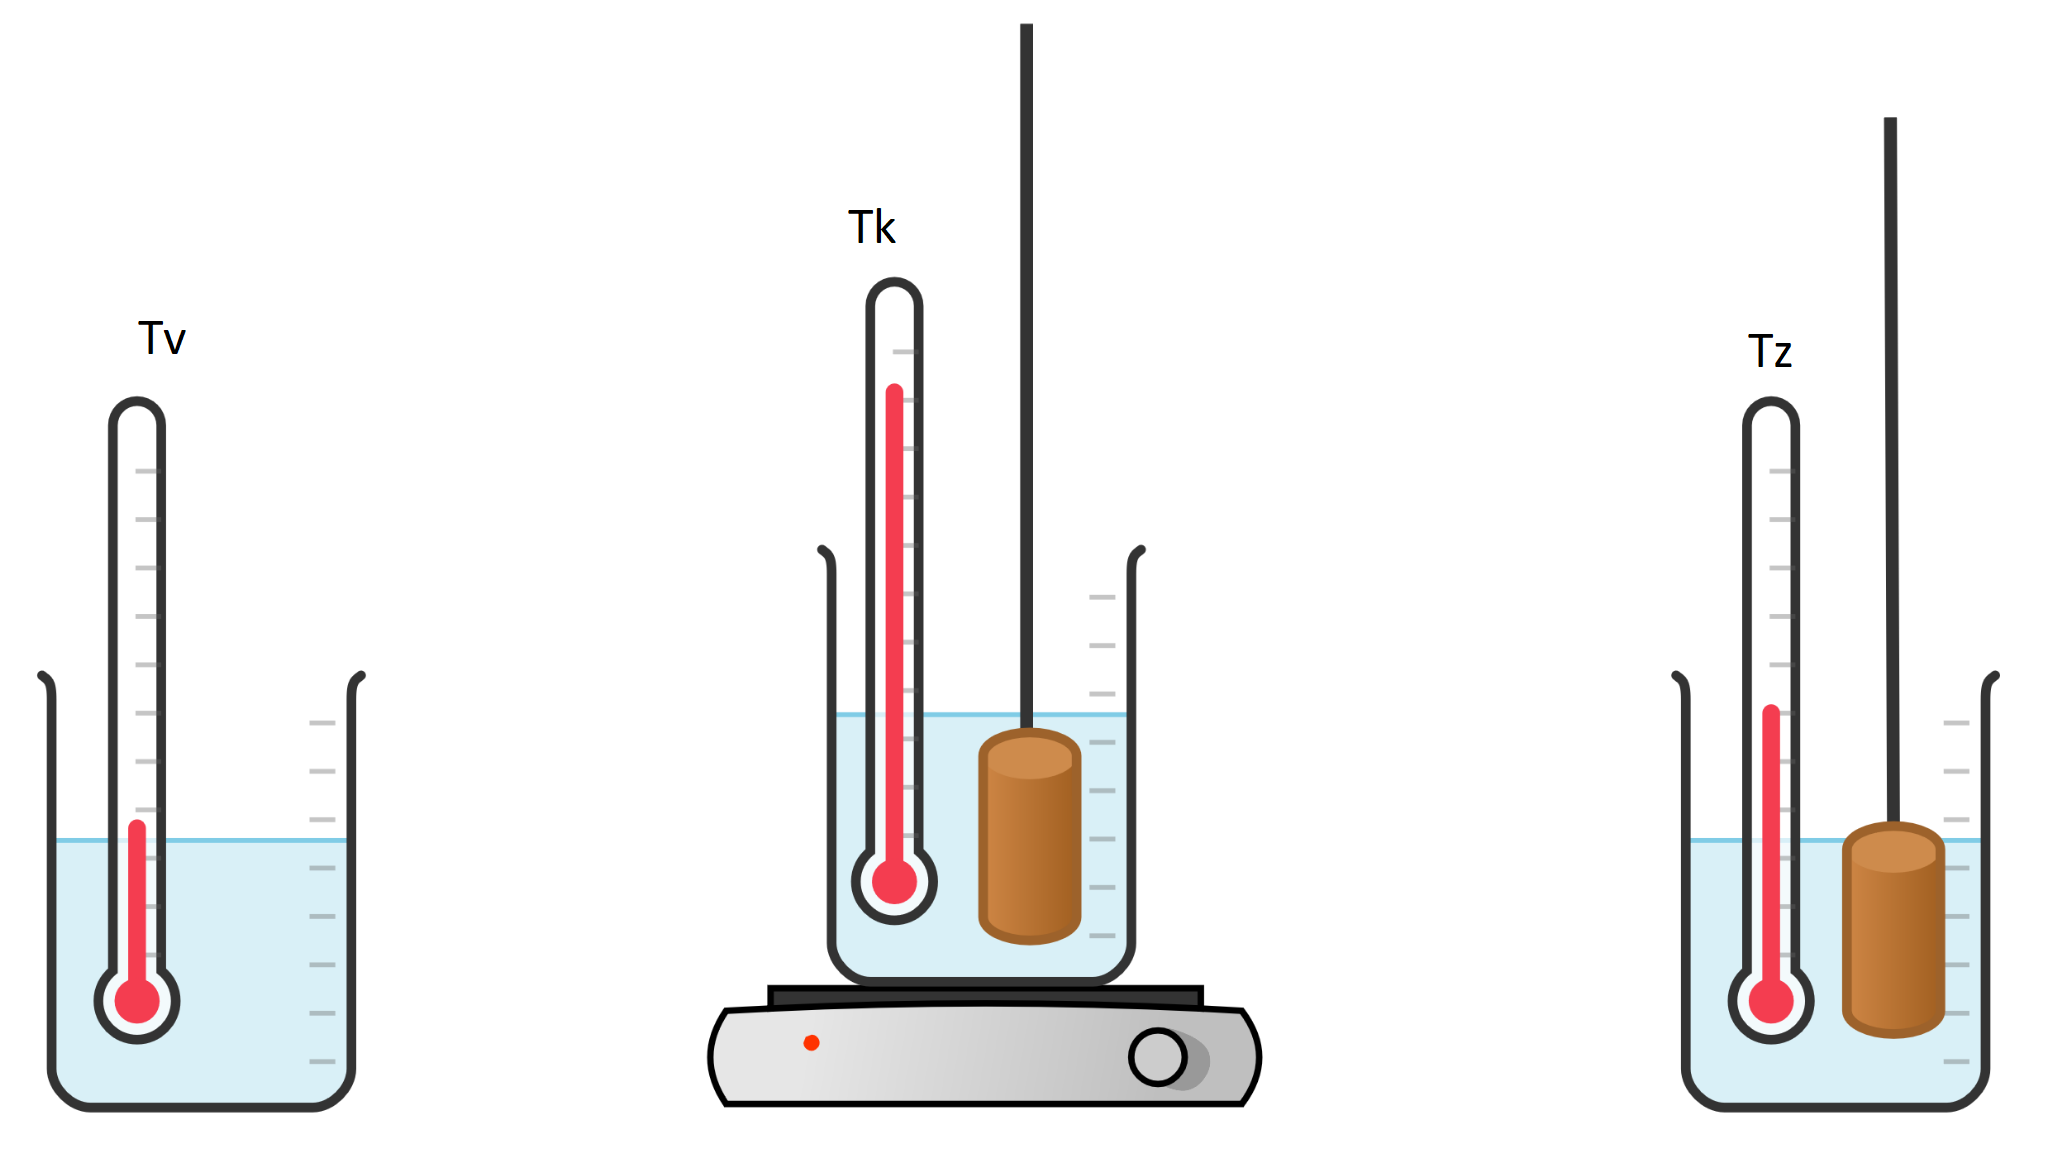
\includegraphics[scale=0.5]{skica.png}

\section*{Meritve:}

Vzemi 150 ml hladne vode in ji izmero temperaturo $T_v.$ V vodo previdno položi kovino, ki smo jo prej segreli v vodi in predpostavimo, da ima na začetku enako temperaturo $T_k$  kot segreta voda. Vodo, v kateri je kovina, večkrat premešaj. Počakaj, da se temperatura ustali in odčitaj njeno vrednost $T_z$. Meritve zapisuj v tabelo. Vsako meritev ponovi trikrat. Postopek ponovi še za preostale tri kovine.

\begin{multicols}{2}

\begin{table}[H]
\centering
\renewcommand{\arraystretch}{1.5}
\begin{tabular}{llllll}
   & & \multicolumn{1}{c}{Al} & & \multicolumn{1}{c}{$\overline{T}$} & \multicolumn{1}{c}{$\Delta T$} \\
   \hline
$T_k [^\circ C]$ & 97,4     & 90,5    & 95,7    & 94,5                    & 4,0                     \\
\hline
$T_z [^\circ C]$ & 39,1     & 36,8    & 38,6    & 38,2                    & 1,4                     \\
\hline
$T_v [^\circ C]$ & 25,5     & 26,4    & 26,5    & 26,1                    & 0,6 \\
\hline
\end{tabular}
\end{table}

\begin{table}[H]
\centering
\renewcommand{\arraystretch}{1.5}
\begin{tabular}{llllll}
   & & \multicolumn{1}{c}{Pb} & & \multicolumn{1}{c}{$\overline{T}$} & \multicolumn{1}{c}{$\Delta T$} \\
   \hline
$T_k [^\circ C]$ & 96,7 & 91,4 & 97,1 & 95,1 & 3,6 \\
\hline
$T_z [^\circ C]$ & 27,4 & 26,4 & 28,1 & 27,3 & 0,9 \\
\hline
$T_v [^\circ C]$ & 25,6 & 23,8 & 26,4 & 25,3 & 1,4 \\
\hline
\end{tabular}
\end{table}

\columnbreak

\begin{table}[H]
\centering
\renewcommand{\arraystretch}{1.5}
\begin{tabular}{llllll}
   & & \multicolumn{1}{c}{Cu} & & \multicolumn{1}{c}{$\overline{T}$} & \multicolumn{1}{c}{$\Delta T$} \\
   \hline
$T_k [^\circ C]$ & 97,0 & 90,1 & 95,8 & 94,3 & 4,2 \\
\hline
$T_z [^\circ C]$ & 30,3 & 30,0 & 31,9 & 30,8 & 1,2 \\
\hline
$T_v [^\circ C]$ & 25,9 & 24,2 & 26,6 & 25,5 & 1,3 \\
\hline
\end{tabular}
\end{table}

\begin{table}[H]
\centering
\renewcommand{\arraystretch}{1.5}
\begin{tabular}{llllll}
   & & \multicolumn{1}{c}{Fe} & & \multicolumn{1}{c}{$\overline{T}$} & \multicolumn{1}{c}{$\Delta T$} \\
   \hline
$T_k [^\circ C]$ & 96,6 & 91,3 & 94,5 & 94,2 & 2,8 \\
\hline
$T_z [^\circ C]$ & 30,1 & 33,9 & 34,4 & 32,8 & 2,7 \\
\hline
$T_v [^\circ C]$ & 25,9 & 28,4 & 26,8 & 27,0 & 1,4 \\
\hline
\end{tabular}
\end{table}

\end{multicols}
\section*{Rezultati in obdelava podatkov:}

\begin{multicols}{2}
$c_u$ lahko izmerimo s pomočjo formule:
\begin{equation}
   c_k = \frac{m_v c_v (T_z - T_v)}{m_k (T_k - T_z)}
\end{equation}

\columnbreak

Kjer lahko uporabimo parametre:
\begin{gather}
   m_k = 200g \\
   m_v = 150g \\
   c_v = 4200 \frac{J}{kgK}
\end{gather}

\end{multicols}

Iz tega sledijo rezultati:
\begin{table}[H]
   \centering
   \renewcommand{\arraystretch}{1.5}
   \begin{tabular}{lllllll}
      & $c_{u1}[\frac{J}{kgK}]$ & $c_{u2}[\frac{J}{kgK}]$ & $c_{u3}[\frac{J}{kgK}]$ & $\overline{c_u}[\frac{J}{kgK}]$ & $\Delta c_u[\frac{J}{kgK}]$ & $\delta c_u$ \\
      \hline
   Al & 734,8    & 610,1   & 667,5   & 670,8                   & 64,0                    & 9,5\%  \\
Pb & 81,8     & 126,0   & 77,6    & 95,1                    & 30,9                    & 32,4\% \\
Cu & 207,8    & 304,0   & 261,3   & 257,7                   & 49,9                    & 19,4\% \\
Fe & 198,9    & 301,8   & 398,3   & 299,7                   & 100,8                   & 33,6\%
   
   \end{tabular}
   \end{table}

Te rezultate lahko primerjamo tudi z rezultati iz literature:
\begin{table}[H]
   \centering
   \renewcommand{\arraystretch}{1.5}
   \begin{tabular}{llll}
      & ekspriment $[\frac{J}{kgK}]$ & literatura $[\frac{J}{kgK}]$ & $\delta $ \\
      \hline
      Al & 670,8 & 880 & 23,8\% \\
      Pb & 95,1  & 130 & 26,8\% \\
      Cu & 257,7 & 390 & 33,9\% \\
      Fe & 299,7 & 500 & 40,1\%
   \end{tabular}
   \end{table}


\section*{Interpretacija:}

Relativna napak tako meritev kot tudi razlike do rezultatov iz literature so velike. 
Za začetek so lahko tukaj napake pri kalibraciji in odčitavanju termometrov in razlike v temperaturi kovni v primerjavi z vodo v kateri so se kovine grele. Nadaljnjo lahko podvomimo v čistost zlitin, ki imajo lahko velik vpliv na toplotno prevodnost. Potem so tukaj še izgube skozi stene in v zrak preko izhlapevanja vode. 

Iz tega bi se dalo zaključiti, da bi bilo bolje uporabiti drugačen način merjenja specifične toplote snovi od tukaj demonstriranega.

\end{document}